%%%%%%%%%%%%%%%%%%%%%%%%%%%%%%%%%%%%%%%%%%%%%%%%%%%%%%%%%
\section{Scenario}
\label{sec:scenario}

The tests take place in the \iterm{RoboCup@Home arena}. Nonetheless, some tests can take place outside the arena, in a previously unknown public place. Rules in this section are related to the \iterm{RoboCup@Home arena} and its contents.

\subsection{RoboCup@Home arena}
The \iterm{RoboCup@Home arena} is a realistic home setting (apartment) consisting of inter-connected rooms.
The minimal configuration consists of
\begin{itemize}
	\item bedroom,
	\item dining room,
	\item living room, and
	\item kitchen.
\end{itemize}
Depending on the Local Organization, there may be multiple apartments which may be different to each other.
Robot must be prepared to perform any task in any arena, not the same arena every time.

The arena is decorated and dressed to resemble a typical apartment in the hosting country, including all necessities and decorations one can find in a normal house.
Please do note that what is considered as \enquote{normal} may greatly vary by culture and on the location where the RoboCup event is hosted.
Decorations include, but are not limited to: plants, mirrors, paintings, posters, plates, picture frames, wall clocks, candles with holders, and books.
For a description of objects, please refer to \refsec{rule:scenario_objects}

\subsection{Walls, doors and floor}
\label{rule:scenario_walls}

The indoor home setting will be surrounded by high and low \Term{walls}{Arena walls}.
These walls will be built up using standard fair construction material.

\begin{enumerate}
	\item \textbf{Walls:} Walls have a minimum height of \SI{60}{\centi\meter}. A maximum height is not specified, but must allow the audience to watch the competition.\\
	Walls are fixed and not to be modified during the competition (see~\refsec{rule:scenario_changes}).

	\item \textbf{Doors:} There will be at least two \Term{doors}{Arena doors}, an entrance and an exit, to be used as starting points for the robots (see~\refsec{rule:start_position}).
	% At least one of the entrances will be a door with a handle (not a knob).\
	Inside the arena rooms are connected by doors (at least one).
	All doors have handles, not knobs.
	Doors can be closed at any time, and it is expected that robots be able to open them.

	\item \textbf{Floor:} The floor of the arena as well as the doorways of the arena are even.
	That is, there will be no significant steps or even stairways.
	However, minor unevenness such as carpets, transitions in floor covering between different areas, and minor gaps (especially at doorways) can be expected.

	\item \textbf{Appearance:} Floor and walls are mainly uni-colored but can contain texture, e.g., a carpet on the floor, or a poster or picture on the wall.\\
	Although being unlikely at the moment, transparent elements are also possible.
\end{enumerate}


\subsection{Furniture}
\label{rule:scenario_furniture}
The arena will be equipped with typical objects (furniture) that are not specified in quantity and kind.

The minimal configuration consists of:
\begin{itemize}
	\item a bed,
	\item a couch,
	\item a small table,
	\item a small dinner table with two chairs,
	\item an open cupboard or small table with a television and remote control,
	\item a cupboard with drawers, and
	\item a bookcase or shelf with doors and some books inside
\end{itemize}

Likewise the arena's kitchen must have:
\begin{itemize}
	\item a dishwasher,
	\item a microwave,
	\item a sink, and
	\item a refrigerator in the kitchen (with some cans and plastic bottles inside).
\end{itemize}

A typical arena setup is shown in~\reffig{fig:scenario_arena}.

\begin{figure}[tbp]
	\centering
	\subfloat[Typical arena]{\label{fig:scenario_arena}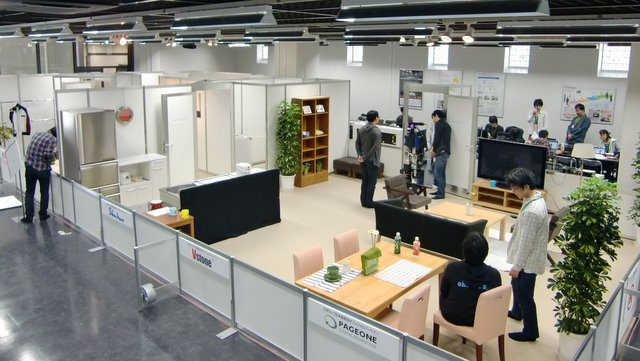
\includegraphics[height=46mm]{images/typical_arena.jpg}} ~
	\subfloat[Typical objects]{\label{fig:scenario_objects}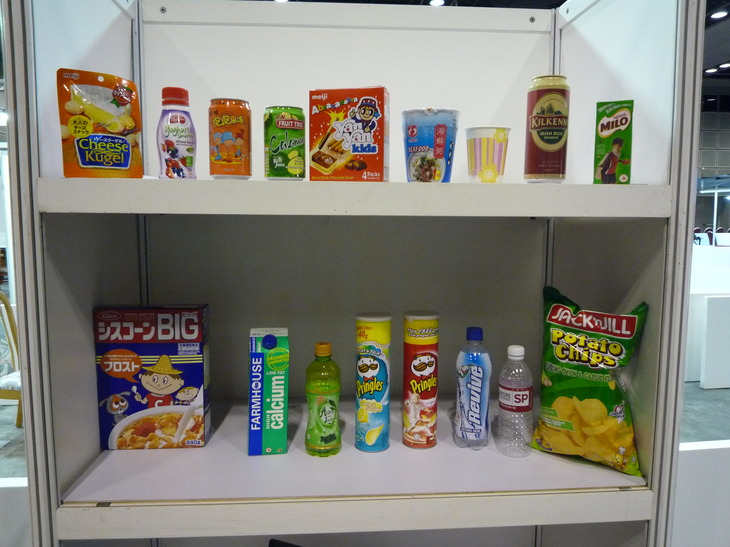
\includegraphics[height=46mm]{images/typical_objects.jpg}}
	\caption{Scenario examples: (a) a typical arena, and (b) typical objects.}
	\label{fig:arena}
\end{figure}


\subsubsection{Cupboard}
The cupboard can be any shelf-like furniture in which objects can be placed.
\begin{itemize}
	\item[\textbf{Doors:}] The cupboard may have doors.
	\item[\textbf{Drawers:}] The cupboard must have at least two drawers betweem 90cm and 120cm from floor level.
	\item[\textbf{Shelves:}] The minimum distance between shelf or layers is 30cm.
\end{itemize}

\subsubsection{Shelf}
A shelf, rack, or bookcase is required in RoboCup@Home.
The shelf can be any shelf-like furniture in which objects can be placed.
\begin{itemize}
	\item[\textbf{Doors:}] The shelf must have at least one door (preferrably a vertical one) covering up to one half of it.
	\item[\textbf{Drawers:}] The shelf must have no drawers.
	\item[\textbf{Shelves:}] The shelf must have 5 shelves or layers between 0.0m and 1.80m from the ground, with a minimum distance of 30cm between shelves or layers.
\end{itemize}

\subsubsection{Fridge}
Fridges must not be smaller than 120m. At least one powered and functioning fridge is required.


\subsection{Changes to the arena}
\label{rule:scenario_changes}

Since the robots should be able to function in the real world the scenario is not fixed and might change without further notice.
\begin{enumerate}
	\item \textbf{Major changes:}
	The arena is meant to be a simulated apartment.
	The furniture might be moved around between tests.
	This includes furniture that is a named location (see~\refsec{rule:scenario_names}).
	As in a normal home, furniture is not very likely to move from one room to another and is unlikely to be moved to the other side of a room.
	However, a couch or table may be rotated, moved to its side etc.
	Walls will stay in place and rooms will not change function.
	Passages might be blocked and cleared.
	One hour before a test slot begins no \iterm{major changes} will be made.
	This time will be shortened in the future.

	\item \textbf{Minor changes:} In contrast to major changes, \iterm{minor changes} like, for instance, slightly moved chairs cannot be avoided and may happen at any time (even during a test).
\end{enumerate}


%%%%%%%%%%%%%%%%%%%%%%%%%%%%%%%%%%%%%%%%%%%%%%%%%%%%%%%%%%%%%%%%%%
%
% Objects section.
%
% Revisited by Mauricio Matamoros for 2015
%
%%%%%%%%%%%%%%%%%%%%%%%%%%%%%%%%%%%%%%%%%%%%%%%%%%%%%%%%%%%%%%%%%%
\def\NumObjects{30\ }
\def\NumLocations{20\ }
\def\NumNames{20\ }

\subsection{Objects}
\label{rule:scenario_objects}
Some tests in the RoboCup@Home league involve recognizing and manipulating \iterm{objects}(See~\reffig{fig:scenario_objects}).
The TC will compile a list of at least \NumObjects objects for this purpose, assigning them official names.
Most objects are likely to be lightweight and easy to grasp with one hand.
Each object has assigned a category (e.g. an \textit{apple} and a \textit{banana} belong to the \textit{fruits} category).
Each \iterm{object category} has assigned a \iterm{predefined location} (e.g. an \textit{fruits} can be found in the \textit{kitchen table}).
Assignments are announced during setup days (See~\refsec{chap:setup_and_preparation}).
An exemplar of each object is provided before the competition for training.

There are two types of objects:

\begin{enumerate}
	\item \textbf{\iterm{Known objects}:} Objects previously known by the robot and that it can identify and manipulate.
	There are two kinds of known objects:
	\begin{enumerate}
		\item \textbf{\iterm{Regular objects}:} Objects with no noticeable difference among peers (e.g.~soda can, cereal box, cutlery, etc).
		\item \textbf{\iterm{Alike objects}:} Objects which are different one from another, but still considered by people to be the same (e.g.~apple, sandwich, cloth, etc.).
	\end{enumerate}

	\item \textbf{\iterm{Unknown objects}:} Any other object that is not known beforehand but can be grasped or handled.
\end{enumerate}

\subsection{List of Predefined Objects}
\label{rule:scenario_objects_list}
The minimal configuration consists of:
\begin{itemize}
	\item \textbf{\iterm{Tableware}:} Dish, bowl, cup (or mug), and napkin.
	\item \textbf{\iterm{Cutlery}:} Fork, knife, and spoon.
	\item \textbf{\iterm{Bags}:} Lightweight. With stiff, vertical handles.
	\item \textbf{\iterm{Trays}:} A transport object like a tray or basket. Intended for two-handed manipulation.
	\item \textbf{\iterm{Pourable}:} An object whose content can be poured (e.g. muesli, cereal, etc.).
	\item \textbf{\iterm{Heavy object}:} Weight between 1.0kg and 1.5kg).
	\item \textbf{\iterm{Tiny object}:} A lightweight object with no bigger than 5cm (e.g. paper, teabag, pen).
	\item \textbf{\iterm{Fragile object}:} An easy-to-break object, (e.g. chocolate egg).
	\item \textbf{\iterm{Amorphous object}:} An flexible object that may take an infinite number of shapes (e.g. cloth, magnetic puzzle, etc.).
\end{itemize}

\paragraph*{Important note:} It is not allowed to modify any of the objects provided for training.
Teams are not allowed to keep more than 5 the objects provided for training at a time nor retaining it for more than one hour.

\begin{figure}[H]
	\centering
	\subfloat[Bright-colored paper bags]{
		\label{fig:scenario_container_bag}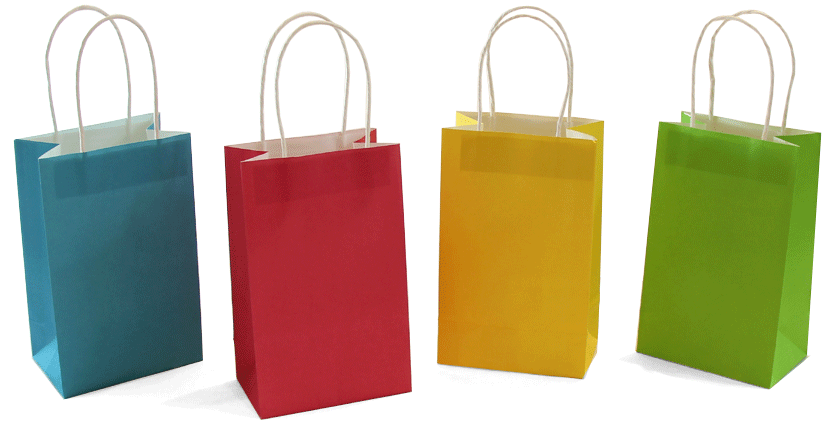
\includegraphics[width=0.33\textwidth]{images/container_paper_bag.png}}~
	\subfloat[Cereal bowls]{
		\label{fig:scenario_container_bowl}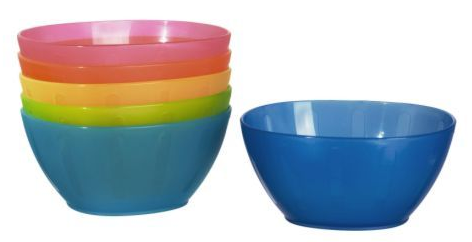
\includegraphics[width=0.33\textwidth]{images/container_bowl.png}}~
	\subfloat[Serving tray]{
		\label{fig:scenario_container_tray}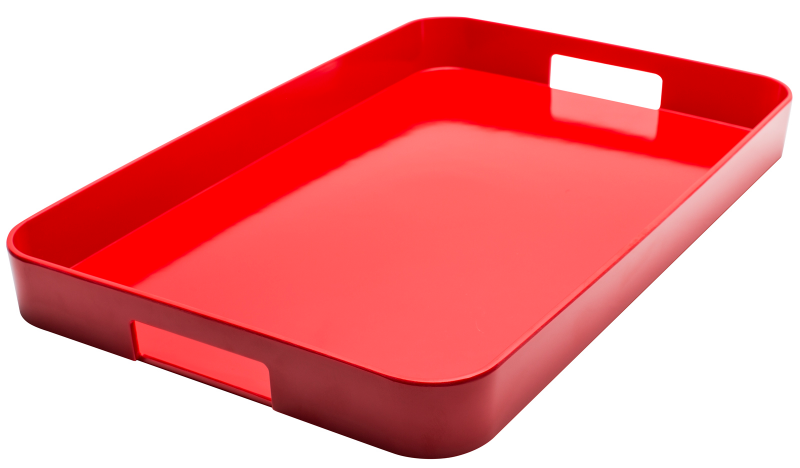
\includegraphics[width=0.33\textwidth]{images/container_tray.png}}
	\caption{Example of object containers}
	\label{fig:scenario_containers}
\end{figure}

\subsection{Attributes of Predefined Objects}
\label{rule:scenario_objects_attributes}
During the competition, objects can be requested based on their category \iterm{object category}, its physical attributes, or a combination of both.
Relevant attributes to be used are:
\begin{itemize}
	\item Color (e.g. red, blue, black with white dots, etc.).
	\item Relative estimated size (smallest, largest, big one, etc.).
	\item Relative estimated weight (lightest, heaviest).
	\item Relative position (left of, right most, etc.).
	\item Object description (is fragile, is container, can be poured, requires two hands, etc.).
\end{itemize}

\noindent\textbf{Remark:} Measurements are estimations and based on common sense. It is OK for robots to consider similar objects to be about the same size or weight.

%%%%%%%%%%%%%%%%%%%%%%%%%%%%%%%%%%%%%%%%%%%%%%%%%%%%%%%%%%%%%%%%%%
%
% Predefined locations section.
%
%%%%%%%%%%%%%%%%%%%%%%%%%%%%%%%%%%%%%%%%%%%%%%%%%%%%%%%%%%%%%%%%%%

\subsection{Predefined rooms and locations}
\label{rule:scenario_locations}
Some tests in the RoboCup@Home league involve \iterm{predefined locations} where people or objects can be found.
The TC will compile a list of predefined locations that may include furniture (e.g. bookshelf), decorations (e.g. plant, mirror), and doors.
Each \iterm{predefined location} has assigned a \iterm{location class} (e.g. an \textit{coach} and a \textit{arm chair} belong to the \textit{seat} class).
Room names, predefined locations, and location classes are announced during setup days (See~\refsec{chap:setup_and_preparation}).



\subsection{Predefined (person) names}\label{rule:scenario_names}
Some tests in the RoboCup@Home league involve memorizing a person name.
All people in the arena has an assigned \iterm{predefined name}.
The TC will compile a list of \NumNames \iterm{predefined names}.
The names are \SI{25}{\percent} male, \SI{25}{\percent} female, and \SI{50}{\percent} gender-neutral, taken from the list of most common used names in the United States.
Predefined names are announced during setup days (See~\refsec{chap:setup_and_preparation}).


\subsection{Wireless network}
\label{rule:scenario_wifi}

For wireless communication, an \iterm{arena network} is provided. The actual infrastructure depends on the local organization.
The organizers do NOT guarantee reliability and performance of wireless communication.
Teams required to start must do so regardless the availability of the network infrastructure.

The following rules apply:

\begin{itemize}
	\item Only the \iterm{arena network} can be used during tests.
	\item During the competitions, only the active team is allowed to use the \iterm{arena network}.
	\item The \iterm{arena network} provides one Virtual Local Area Networks (VLANs) per team.
	\item Each VLAN is most likely to have its own SSID/password.
	\item VLAN traffic is separated from any other team, routed to the team's network cable (team area).
	\item Each VLAN is also connected to the Internet.
\end{itemize}

\indent\textbf{Remark:} Teams broadcasting unauthorized (aka rogue) wireless networks will be disqualified from the competition, and have their devices confiscated by the OC.
This includes smartphones and concealed SSIDs.
It is advised to verify your devices.


% Local Variables:
% TeX-master: "../Rulebook"
% End:
